% ex: ts=2 sw=2 sts=2 et filetype=tex
% SPDX-License-Identifier: CC-BY-SA-4.0

\question Usa la siguiente cuadricula para resolver los siguientes incisos:

  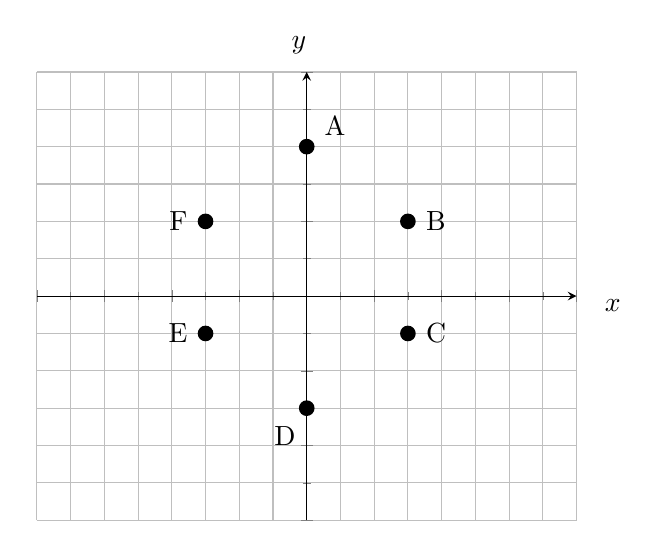
\begin{tikzpicture}
    \begin{axis}[grid=both,ymin=-6,ymax=6,xmax=8,xmin=-8,xticklabel=\empty,yticklabel=\empty,
               minor tick num=1,axis lines = middle,xlabel=$x$,ylabel=$y$,
               label style = {at={(ticklabel cs:1.1)}}]
      \node[label={10:{A}},circle,fill,inner sep=2pt] at (axis cs:0,4) {};
      \node[label={0:{B}},circle,fill,inner sep=2pt] at (axis cs:3,2) {};
      \node[label={0:{C}},circle,fill,inner sep=2pt] at (axis cs:3,-1) {};
      \node[label={260:{D}},circle,fill,inner sep=2pt] at (axis cs:0,-3) {};
      \node[label={180:{E}},circle,fill,inner sep=2pt] at (axis cs:-3,-1) {};
      \node[label={180:{F}},circle,fill,inner sep=2pt] at (axis cs:-3,2) {};
    \end{axis}
  \end{tikzpicture}

  \begin{parts}
    \part Encuentra las coordenadas de los vértices en el polígono. \\
    A(\fillin[0] ,\fillin[4] ) \enspace B(\fillin[3] ,\fillin[2] ) \\
    C(\fillin[3] ,\fillin[-1] ) \enspace D(\fillin[0] ,\fillin[-3] ) \\
    E(\fillin[-3] ,\fillin[-1] ) \enspace F(\fillin[-3] ,\fillin[2] ) \\
    \part Determina el cuadrante en el que se ubica los puntos: \\
    El punto B esta en el cuadrante:\fillin[1]\\
    El punto C esta en el cuadrante:\fillin[4]\\
    El punto E esta en el cuadrante:\fillin[3]\\
    El punto F esta en el cuadrante:\fillin[2]\\
    \part Sacar la distancia entre los puntos: \\
    AB \fillin[$\sqrt{13} = 3.6$] \enspace BC \fillin[3] \enspace CD \fillin[$\sqrt{13} = 3.6$] \\
    DE \fillin[$\sqrt{13} = 3.6$] \enspace EF \fillin[3] \enspace FA \fillin[$\sqrt{13} = 3.6$] \\
    \part Calcula el perímetro de la figura resultante.
      \begin{solution}
        El perímetro es: 20.4
      \end{solution}
  \end{parts}
